% TODO: would benefit from more of a third person writing prose.
% i.e: we are currently talking in terms of "we did X and found Y" rather than
% "because of hyp Z, we tried X and found Y, shown in fig A"
% feels a bit "aimless" of a scientific approach.

\subsection{Unconditional Image Generation}
\label{subsec:evaluationUnconditional}

We evaluate our method on the task of unconditional image generation on datasets
FFHQ256, FFHQ1024, CelebA, LSUN Churches, and LSUN Bedrooms. For LSUN we use
pretrained \gls{vqgan} checkpoints provided by~\cite{bondtaylor2021unleashing},
and for all other unconditional experiments we use checkpoints from the original
work~\cite{esser2021taming}. We evaluate in terms of raw perceptual quality and
coverage, as well as how these metrics are affected by the various
hyperparameters of our model and parameters of the sampling process -- the
latter of which we found to be highly configurable.

\begin{figure}[ht!]
    \centering
    \begin{subfigure}[b]{0.33\textwidth}
        \centering
        \resizebox{\textwidth}{!}{
            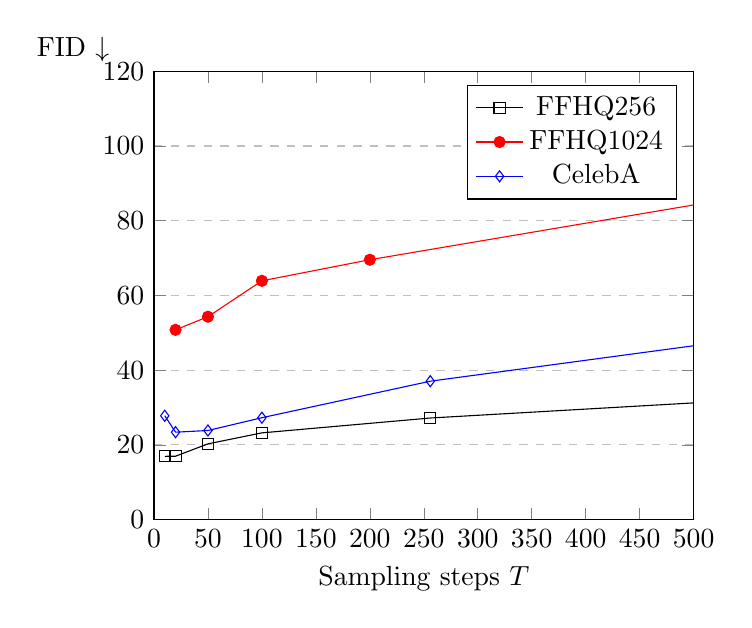
\begin{tikzpicture}
\begin{axis}[
y label style={at={(axis description cs:-0.15,1.0)},rotate=-90,anchor=south},
title={},
xlabel={Sampling steps $T$},
ylabel={FID $\downarrow$},
xmin=0, xmax=500,
ymin=0, ymax=120,
xtick={0,50,100,150,200,250,300,350,400,450,500},
ytick={0,20,40,60,80,100,120},
legend pos=north east,
ymajorgrids=true,
grid style=dashed,
]\addplot[color=black, mark=square]
coordinates {(10.0, 16.933240853331633)(20.0, 16.968015496794585)(50.0, 20.269439432847413)(100.0, 23.214299375538577)(256.0, 27.189009006094718)(512.0, 31.435942790814245)};
\addlegendentry{FFHQ256}
\addplot[color=red, mark=*]
coordinates {(20.0, 50.79169256114352)(50.0, 54.30311107720983)(100.0, 63.90726480083863)(200.0, 69.5533429056805)(512.0, 84.80617604620527)(1024.0, 100.93734948403663)};
\addlegendentry{FFHQ1024}
\addplot[color=blue, mark=diamond]
coordinates {(10.0, 27.79389706651663)(20.0, 23.397719254573232)(50.0, 23.845846223411986)(100.0, 27.26720576724899)(256.0, 37.0436486740923)(512.0, 46.99500404006332)};
\addlegendentry{CelebA}
\end{axis}
\end{tikzpicture}

        }
        \caption{Steps vs. FID}
    \end{subfigure}
    \hfill
    \begin{subfigure}[b]{0.33\textwidth}
        \centering
        \resizebox{\textwidth}{!}{
            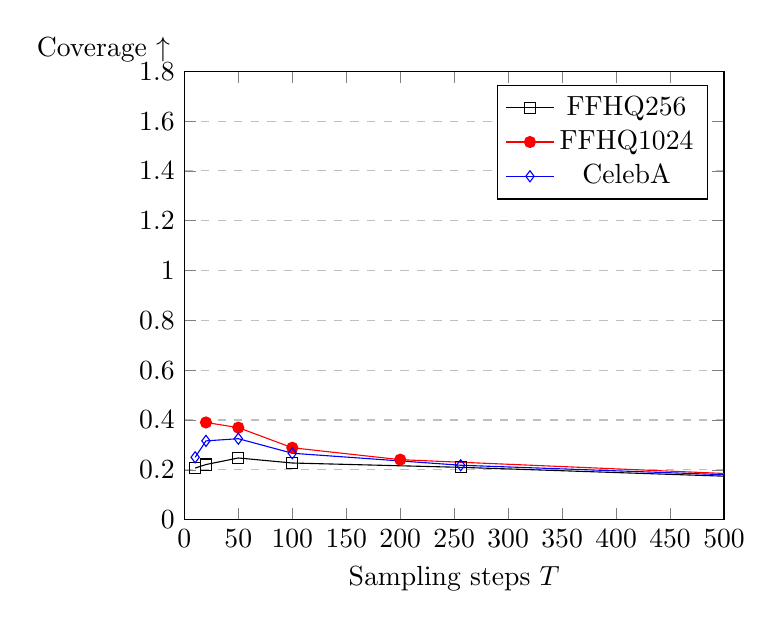
\begin{tikzpicture}
\begin{axis}[
y label style={at={(axis description cs:-0.15,1.0)},rotate=-90,anchor=south},
title={},
xlabel={Sampling steps $T$},
ylabel={Coverage $\uparrow$},
xmin=0, xmax=500,
ymin=0.0, ymax=1.8,
xtick={0,50,100,150,200,250,300,350,400,450,500},
ytick={0.0,0.2,0.4,0.6000000000000001,0.8,1.0,1.2000000000000002,1.4000000000000001,1.6,1.8},
legend pos=north east,
ymajorgrids=true,
grid style=dashed,
]\addplot[color=black, mark=square]
coordinates {(10.0, 0.207)(20.0, 0.221)(50.0, 0.2474)(100.0, 0.2272)(256.0, 0.2098)(512.0, 0.1726)};
\addlegendentry{FFHQ256}
\addplot[color=red, mark=*]
coordinates {(20.0, 0.39)(50.0, 0.3692)(100.0, 0.2884)(200.0, 0.2406)(512.0, 0.183)(1024.0, 0.1448)};
\addlegendentry{FFHQ1024}
\addplot[color=blue, mark=diamond]
coordinates {(10.0, 0.2502)(20.0, 0.316)(50.0, 0.3248)(100.0, 0.2664)(256.0, 0.2182)(512.0, 0.1784)};
\addlegendentry{CelebA}
\end{axis}
\end{tikzpicture}

        }
        \caption{Steps vs. Coverage}
    \end{subfigure}
    \hfill
    \begin{subfigure}[b]{0.33\textwidth}
        \centering
        \resizebox{\textwidth}{!}{
            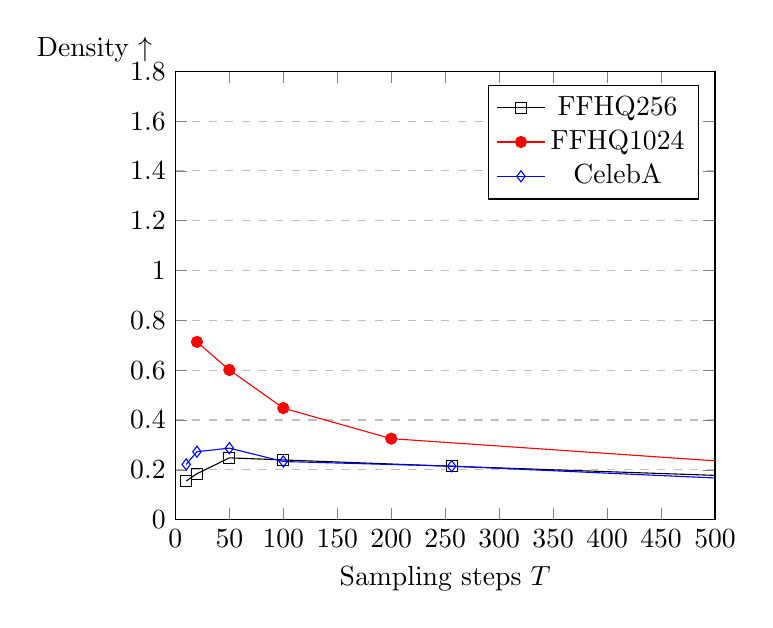
\begin{tikzpicture}
\begin{axis}[
y label style={at={(axis description cs:-0.15,1.0)},rotate=-90,anchor=south},
title={},
xlabel={Sampling steps $T$},
ylabel={Density $\uparrow$},
xmin=0, xmax=500,
ymin=0.0, ymax=1.8,
xtick={0,50,100,150,200,250,300,350,400,450,500},
ytick={0.0,0.2,0.4,0.6000000000000001,0.8,1.0,1.2000000000000002,1.4000000000000001,1.6,1.8},
legend pos=north east,
ymajorgrids=true,
grid style=dashed,
]\addplot[color=black, mark=square]
coordinates {(10.0, 0.155)(20.0, 0.18413333333333332)(50.0, 0.24793333333333334)(100.0, 0.23946666666666666)(256.0, 0.21406666666666666)(512.0, 0.17573333333333332)};
\addlegendentry{FFHQ256}
\addplot[color=red, mark=*]
coordinates {(20.0, 0.7133333333333334)(50.0, 0.6008666666666667)(100.0, 0.44753333333333334)(200.0, 0.3249333333333333)(512.0, 0.2324)(1024.0, 0.16773333333333332)};
\addlegendentry{FFHQ1024}
\addplot[color=blue, mark=diamond]
coordinates {(10.0, 0.2215333333333333)(20.0, 0.2724)(50.0, 0.2869333333333333)(100.0, 0.2332)(256.0, 0.21446666666666664)(512.0, 0.16473333333333331)};
\addlegendentry{CelebA}
\end{axis}
\end{tikzpicture}

        }
        \caption{Steps vs. Density}
    \end{subfigure}
    \caption{
        Plots showing sample quality in terms of different metrics as
        number of sampling steps $\markovSteps$ increases. Counter-intuitively, the
        sample quality decreases with number of sampling steps, seen on
        all metrics and datasets.
    }
\end{figure}

\begin{figure}[ht!]
    \begin{subfigure}[b]{0.33\textwidth}
        \centering
        \resizebox{\textwidth}{!}{
            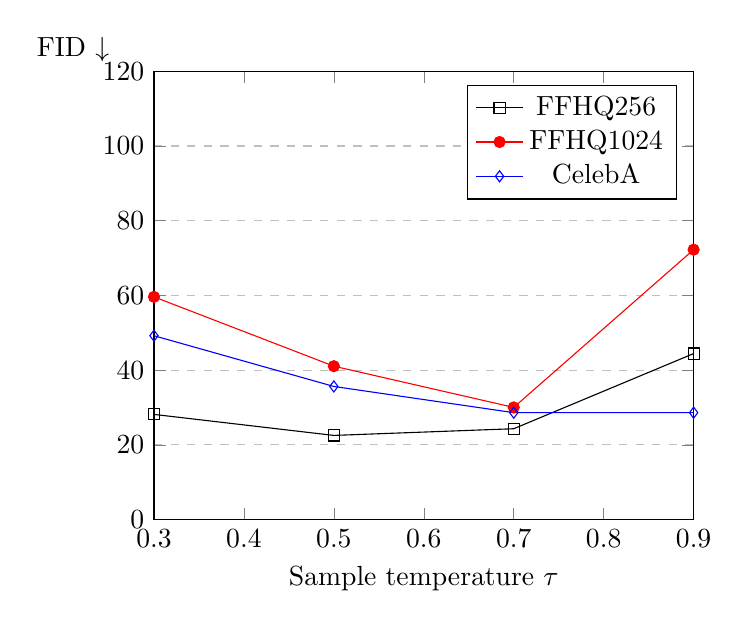
\begin{tikzpicture}
\begin{axis}[
y label style={at={(axis description cs:-0.15,1.0)},rotate=-90,anchor=south},
title={},
xlabel={Sample temperature $\tau$},
ylabel={FID $\downarrow$},
xmin=0.3, xmax=0.9000000000000001,
ymin=0, ymax=120,
xtick={0.3,0.4,0.5,0.6000000000000001,0.7000000000000002,0.8000000000000003,0.9000000000000001},
ytick={0,20,40,60,80,100,120},
legend pos=north east,
ymajorgrids=true,
grid style=dashed,
]\addplot[color=black, mark=square]
coordinates {(1.0, 83.59790014438649)(0.9, 44.43439367176743)(0.7, 24.322136621661407)(0.5, 22.530204016446124)(0.3, 28.155348332963445)};
\addlegendentry{FFHQ256}
\addplot[color=red, mark=*]
coordinates {(1.0, 281.35575866892975)(0.9, 72.24972119845785)(0.7, 30.030630965588852)(0.5, 41.06155796980428)(0.3, 59.61624309496067)};
\addlegendentry{FFHQ1024}
\addplot[color=blue, mark=diamond]
coordinates {(1.0, 75.80203954506536)(0.9, 28.617311837121477)(0.7, 28.621503391331398)(0.5, 35.63571015802388)(0.3, 49.21726306807049)};
\addlegendentry{CelebA}
\end{axis}
\end{tikzpicture}

        }
        \caption{Temperature $\temperature$ vs. FID}
    \end{subfigure}
    \hfill
    \begin{subfigure}[b]{0.33\textwidth}
        \centering
        \resizebox{\textwidth}{!}{
            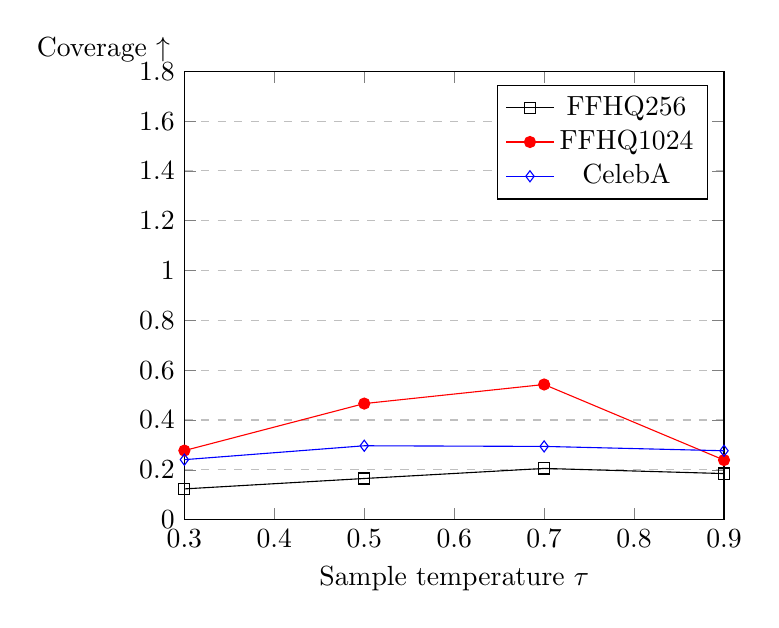
\begin{tikzpicture}
\begin{axis}[
y label style={at={(axis description cs:-0.15,1.0)},rotate=-90,anchor=south},
title={},
xlabel={Sample temperature $\tau$},
ylabel={Coverage $\uparrow$},
xmin=0.3, xmax=0.9000000000000001,
ymin=0.0, ymax=1.8,
xtick={0.3,0.4,0.5,0.6000000000000001,0.7000000000000002,0.8000000000000003,0.9000000000000001},
ytick={0.0,0.2,0.4,0.6000000000000001,0.8,1.0,1.2000000000000002,1.4000000000000001,1.6,1.8},
legend pos=north east,
ymajorgrids=true,
grid style=dashed,
]\addplot[color=black, mark=square]
coordinates {(1.0, 0.0662)(0.9, 0.1848)(0.7, 0.2054)(0.5, 0.165)(0.3, 0.1232)};
\addlegendentry{FFHQ256}
\addplot[color=red, mark=*]
coordinates {(1.0, 0.0004)(0.9, 0.239)(0.7, 0.5424)(0.5, 0.4658)(0.3, 0.277)};
\addlegendentry{FFHQ1024}
\addplot[color=blue, mark=diamond]
coordinates {(1.0, 0.124)(0.9, 0.2764)(0.7, 0.2938)(0.5, 0.2964)(0.3, 0.2406)};
\addlegendentry{CelebA}
\end{axis}
\end{tikzpicture}

        }
        \caption{Temperature $\temperature$ vs. Coverage}
    \end{subfigure}
    \hfill
    \begin{subfigure}[b]{0.33\textwidth}
        \centering
        \resizebox{\textwidth}{!}{
            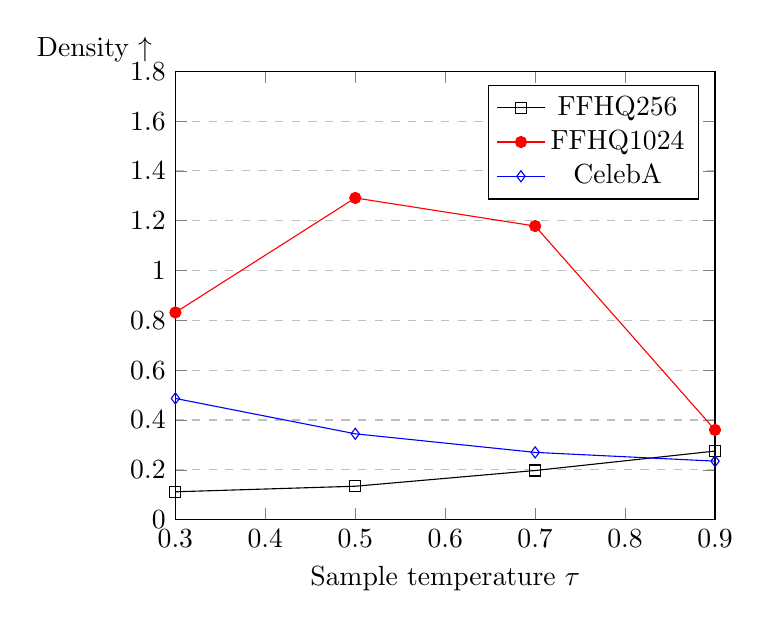
\begin{tikzpicture}
\begin{axis}[
y label style={at={(axis description cs:-0.15,1.0)},rotate=-90,anchor=south},
title={},
xlabel={Sample temperature $\tau$},
ylabel={Density $\uparrow$},
xmin=0.3, xmax=0.9000000000000001,
ymin=0.0, ymax=1.8,
xtick={0.3,0.4,0.5,0.6000000000000001,0.7000000000000002,0.8000000000000003,0.9000000000000001},
ytick={0.0,0.2,0.4,0.6000000000000001,0.8,1.0,1.2000000000000002,1.4000000000000001,1.6,1.8},
legend pos=north east,
ymajorgrids=true,
grid style=dashed,
]\addplot[color=black, mark=square]
coordinates {(1.0, 0.07566666666666666)(0.9, 0.2750666666666667)(0.7, 0.19706666666666664)(0.5, 0.13393333333333332)(0.3, 0.11159999999999999)};
\addlegendentry{FFHQ256}
\addplot[color=red, mark=*]
coordinates {(1.0, 0.00019999999999999998)(0.9, 0.3599333333333333)(0.7, 1.1785333333333332)(0.5, 1.2913999999999999)(0.3, 0.8315333333333333)};
\addlegendentry{FFHQ1024}
\addplot[color=blue, mark=diamond]
coordinates {(1.0, 0.12519999999999998)(0.9, 0.23466666666666663)(0.7, 0.26986666666666664)(0.5, 0.3444666666666667)(0.3, 0.4864)};
\addlegendentry{CelebA}
\end{axis}
\end{tikzpicture}

        }
        \caption{Temperature $\temperature$ vs. Density}
    \end{subfigure}
    \caption{
        Plots showing sample quality in terms of different metrics as sample
        temperature $\temperature$ is changed. Given the other parameters, a good choice
        of $\temperature$ falls in the range $0.5-0.7$. However, this range may
        differ depending on the other choice of parameters.
    }
\end{figure}

\begin{figure}[ht!]
    \begin{subfigure}[b]{0.33\textwidth}
        \centering
        \resizebox{\textwidth}{!}{
            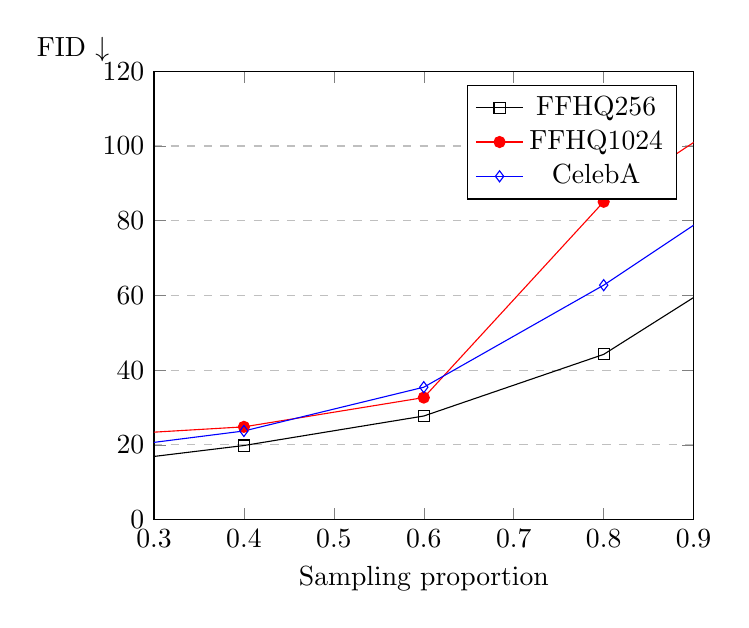
\begin{tikzpicture}
\begin{axis}[
y label style={at={(axis description cs:-0.15,1.0)},rotate=-90,anchor=south},
title={},
xlabel={Sampling proportion},
ylabel={FID $\downarrow$},
xmin=0.3, xmax=0.9000000000000001,
ymin=0, ymax=120,
xtick={0.3,0.4,0.5,0.6000000000000001,0.7000000000000002,0.8000000000000003,0.9000000000000001},
ytick={0,20,40,60,80,100,120},
legend pos=north east,
ymajorgrids=true,
grid style=dashed,
]\addplot[color=black, mark=square]
coordinates {(1.0, 74.66283778948849)(0.8, 44.21927055440783)(0.6, 27.725188336835213)(0.4, 19.825740890874904)(0.2, 13.976620506685805)};
\addlegendentry{FFHQ256}
\addplot[color=red, mark=*]
coordinates {(1.0, 116.81614755529716)(0.8, 85.06652266724691)(0.6, 32.65933412137353)(0.4, 24.82419203797879)(0.2, 21.979835694569083)};
\addlegendentry{FFHQ1024}
\addplot[color=blue, mark=diamond]
coordinates {(1.0, 94.83723271911529)(0.8, 62.7489179950907)(0.6, 35.43514345702618)(0.4, 23.718088259439654)(0.2, 17.614758693266793)};
\addlegendentry{CelebA}
\end{axis}
\end{tikzpicture}

        }
        \caption{Sample proportion vs. FID}
    \end{subfigure}
    \hfill
    \begin{subfigure}[b]{0.33\textwidth}
        \centering
        \resizebox{\textwidth}{!}{
            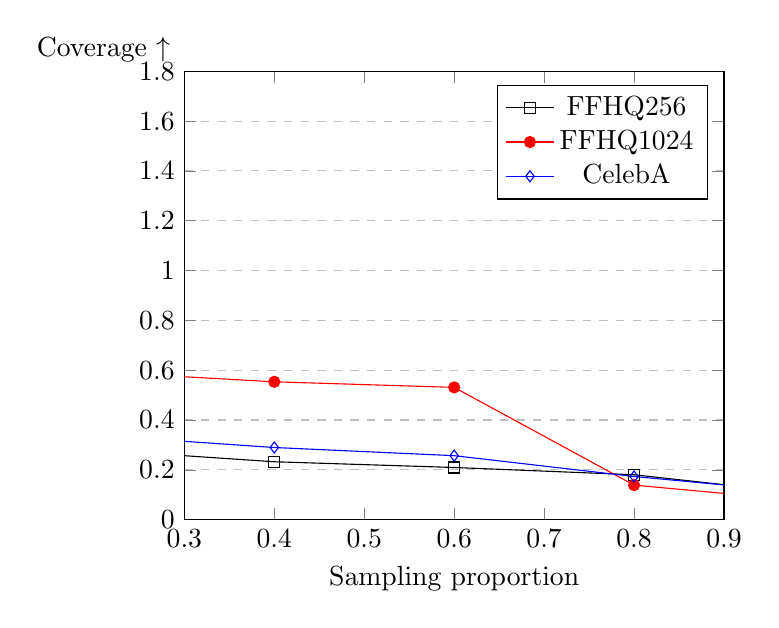
\begin{tikzpicture}
\begin{axis}[
y label style={at={(axis description cs:-0.15,1.0)},rotate=-90,anchor=south},
title={},
xlabel={Sampling proportion},
ylabel={Coverage $\uparrow$},
xmin=0.3, xmax=0.9000000000000001,
ymin=0.0, ymax=1.8,
xtick={0.3,0.4,0.5,0.6000000000000001,0.7000000000000002,0.8000000000000003,0.9000000000000001},
ytick={0.0,0.2,0.4,0.6000000000000001,0.8,1.0,1.2000000000000002,1.4000000000000001,1.6,1.8},
legend pos=north east,
ymajorgrids=true,
grid style=dashed,
]\addplot[color=black, mark=square]
coordinates {(1.0, 0.1002)(0.8, 0.18)(0.6, 0.2092)(0.4, 0.2322)(0.2, 0.2808)};
\addlegendentry{FFHQ256}
\addplot[color=red, mark=*]
coordinates {(1.0, 0.0718)(0.8, 0.1384)(0.6, 0.5308)(0.4, 0.5532)(0.2, 0.5936)};
\addlegendentry{FFHQ1024}
\addplot[color=blue, mark=diamond]
coordinates {(1.0, 0.1054)(0.8, 0.173)(0.6, 0.2566)(0.4, 0.2894)(0.2, 0.3392)};
\addlegendentry{CelebA}
\end{axis}
\end{tikzpicture}

        }
        \caption{Sample proportion vs. Coverage}
    \end{subfigure}
    \hfill
    \begin{subfigure}[b]{0.33\textwidth}
        \centering
        \resizebox{\textwidth}{!}{
            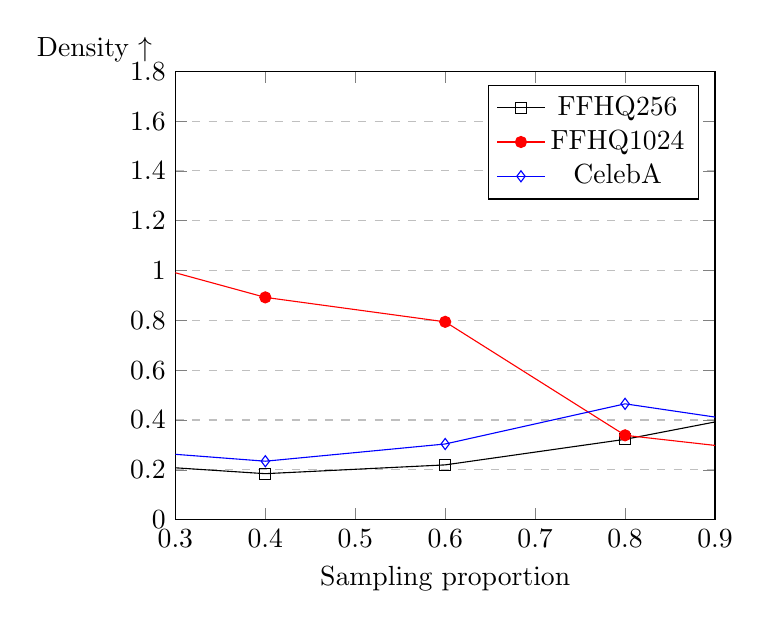
\begin{tikzpicture}
\begin{axis}[
y label style={at={(axis description cs:-0.15,1.0)},rotate=-90,anchor=south},
title={},
xlabel={Sampling proportion},
ylabel={Density $\uparrow$},
xmin=0.3, xmax=0.9000000000000001,
ymin=0.0, ymax=1.8,
xtick={0.3,0.4,0.5,0.6000000000000001,0.7000000000000002,0.8000000000000003,0.9000000000000001},
ytick={0.0,0.2,0.4,0.6000000000000001,0.8,1.0,1.2000000000000002,1.4000000000000001,1.6,1.8},
legend pos=north east,
ymajorgrids=true,
grid style=dashed,
]\addplot[color=black, mark=square]
coordinates {(1.0, 0.46173333333333333)(0.8, 0.32226666666666665)(0.6, 0.21966666666666668)(0.4, 0.18433333333333335)(0.2, 0.23146666666666665)};
\addlegendentry{FFHQ256}
\addplot[color=red, mark=*]
coordinates {(1.0, 0.25726666666666664)(0.8, 0.33840000000000003)(0.6, 0.794)(0.4, 0.8922)(0.2, 1.0897333333333332)};
\addlegendentry{FFHQ1024}
\addplot[color=blue, mark=diamond]
coordinates {(1.0, 0.35853333333333326)(0.8, 0.4648)(0.6, 0.3035333333333333)(0.4, 0.2344)(0.2, 0.2897333333333333)};
\addlegendentry{CelebA}
\end{axis}
\end{tikzpicture}

        }
        \caption{Sample proportion vs. Density}
    \end{subfigure}
    \caption{
        Plots showing sample quality in terms of different metrics as sample
        proportion is changed. Lower values seem to perform better given the
        other parameters, but again the optimal range may differ if other
        parameters are changed.
    }
\end{figure}

\begin{figure}[ht]
    \centering
    \begin{subfigure}[b]{0.47\textwidth}
        \centering
        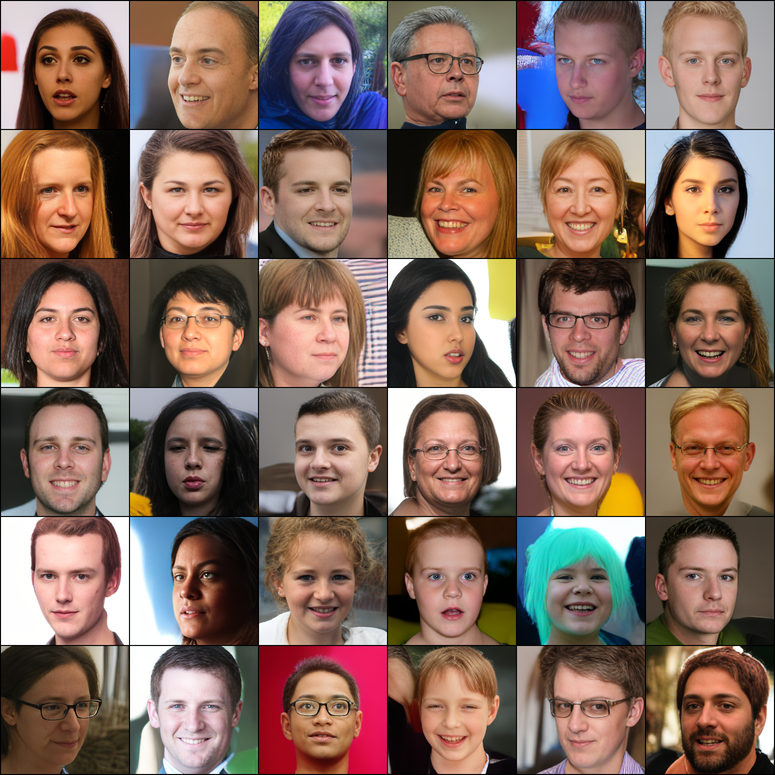
\includegraphics[width=1.0\textwidth]{figures/ffhq256-samples-small.png}
        \caption{
            Non-cherry picked batch of samples from the model trained on FFHQ256.
        }
    \end{subfigure}
    \hfill
    \begin{subfigure}[b]{0.47\textwidth}
        \centering
        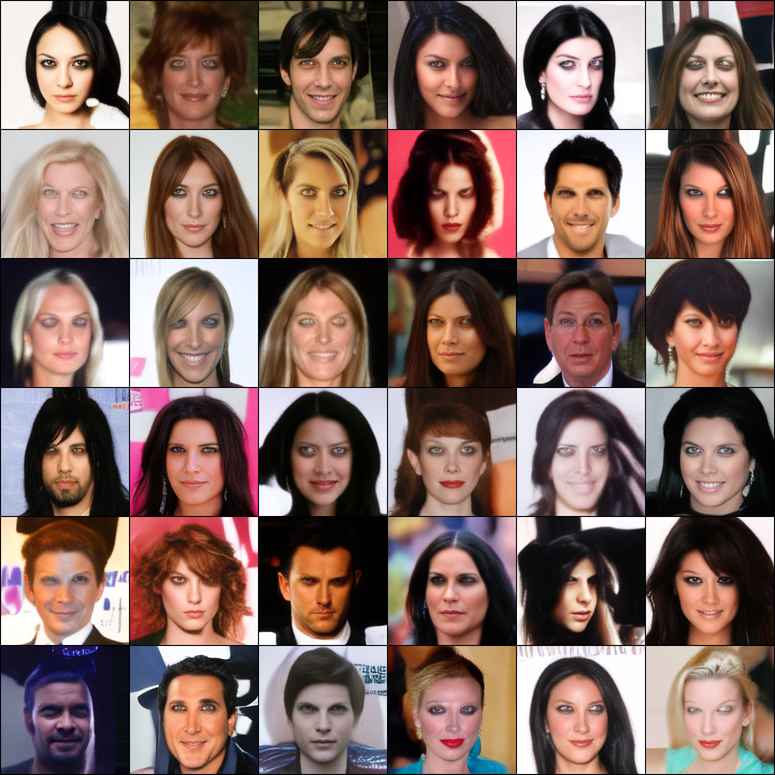
\includegraphics[width=1.0\textwidth]{figures/celeba-samples-small.png}
        \caption{
            Non-cherry picked batch of samples from the model trained on CelebA.
        }
    \end{subfigure}
    \caption{Unconditional generation on $256 \times 256$ face datasets.}
\end{figure}

\begin{figure}[ht]
    \centering
    \begin{subfigure}[b]{\textwidth}
        \centering
        \includegraphics[width=1.0\textwidth]{figures/nearest-ffhq256.png}
        \caption{
            FFHQ256 samples and nearest neighbours from the dataset, based on LPIPS
            perceptual loss. Left-most column is a sample from our trained
            model, followed then by nearest neighbours, increasing in distance
            from left-to-right.
        }
    \end{subfigure}
\end{figure}

\subsection{Conditional Image Generation}

\begin{figure}[ht]
    \centering
    \begin{subfigure}[b]{0.47\textwidth}
        \centering
        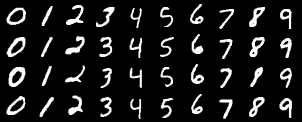
\includegraphics[width=1.0\textwidth]{figures/mnist-samples.png}
        \caption{
            Conditional, pixel-wise generation on MNIST.
        }
    \end{subfigure}
    \hfill
    \begin{subfigure}[b]{0.47\textwidth}
        \centering
        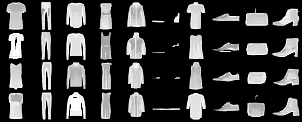
\includegraphics[width=1.0\textwidth]{figures/fashionmnist-samples.png}
        \caption{
            Conditional, pixel-wise generation on Fashion-MNIST.
        }
    \end{subfigure}
    \caption{
        Testing conditional generation using MNIST-style datasets. Coherent
        samples demonstrate that the proposed conditioning method does inject class
        information.
    }
    \label{fig:mnist}
\end{figure}

Another critical component of an ideal generative model is the ability to
control its generation. We explore class-conditioned image generation of
ImageNet at $256 \times 256$ resolution, using the pretrained ImageNet
\gls{vqgan} checkpoints provided by the original work~\cite{esser2021taming}. 

There are many ways to integrate class conditioning to a generative model. One
solution is to pass a one-hot or embedding vector of the classes as an auxiliary
input to the model. We use another simple solution, to add an additional
embedding layer containing one embedding for each of the 1000 classes present in
ImageNet. This approach was done in Image Transformer~\cite{parmar2018image} and
was found to be effective. 

It was not immediately apparent whether this method would also work for
\gls{sundae}, so before running expensive ImageNet experiments we first did some
preliminary experiments on class-conditioned, pixel-wise, \gls{nar} generation
on two MNIST-style datasets: MNIST and Fashion-MNIST. These experiments can be
done, despite not having an associated \gls{vqgan} model, by treating each
possible 8-bit greyscale colour as if it were an index into a discrete codebook
of size $2^8$. Once sampled, we simply output the discrete values directly to
produce a final image. These preliminary experiments showed us that \gls{sundae}
can successfully use class information using this simple approach, seen in
Figure~\ref{fig:mnist}.

\begin{figure}[ht]
    \centering
    \begin{subfigure}[b]{0.47\textwidth}
        \centering
        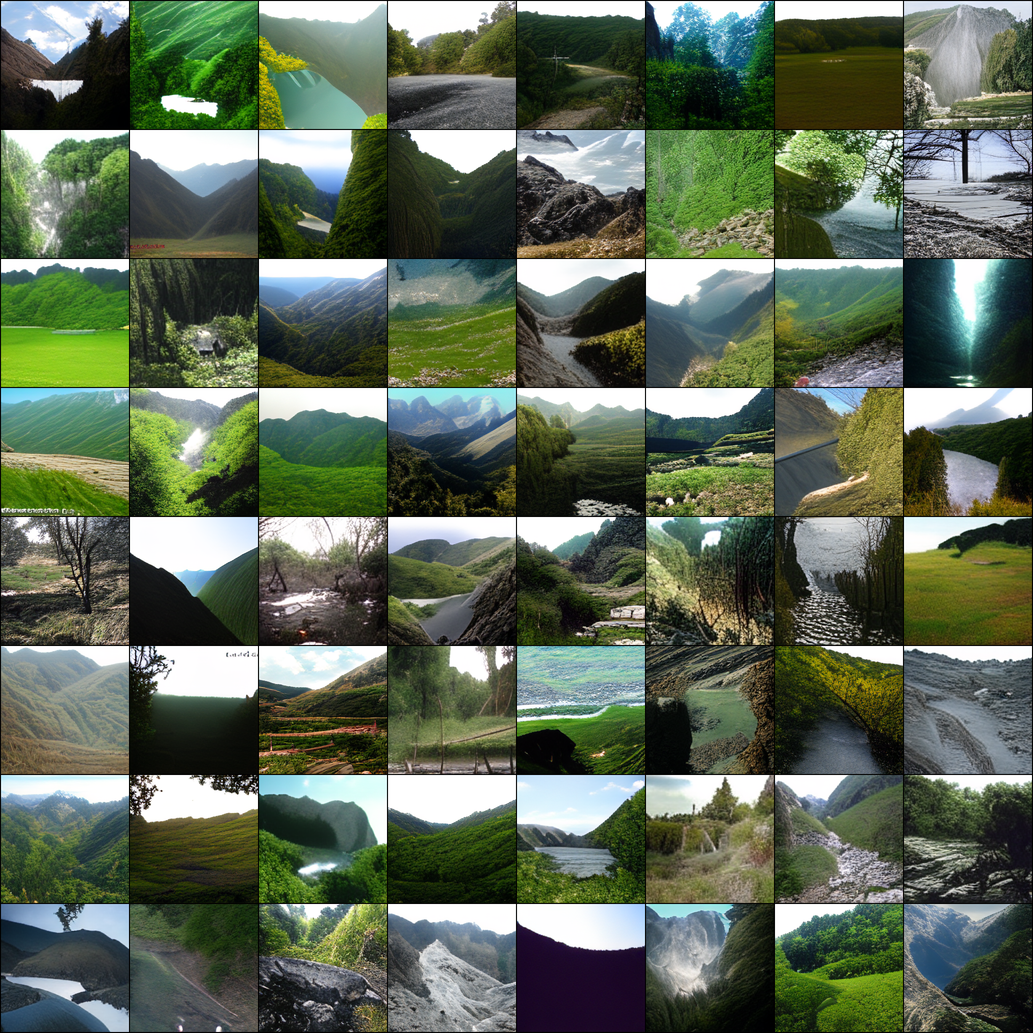
\includegraphics[width=1.0\textwidth]{figures/imagenet-valley-small.png}
        \caption{
            $256 \times 256$ successful samples from the class ``Valley''.}
    \end{subfigure}
    \hfill
    \begin{subfigure}[b]{0.47\textwidth}
        \centering
        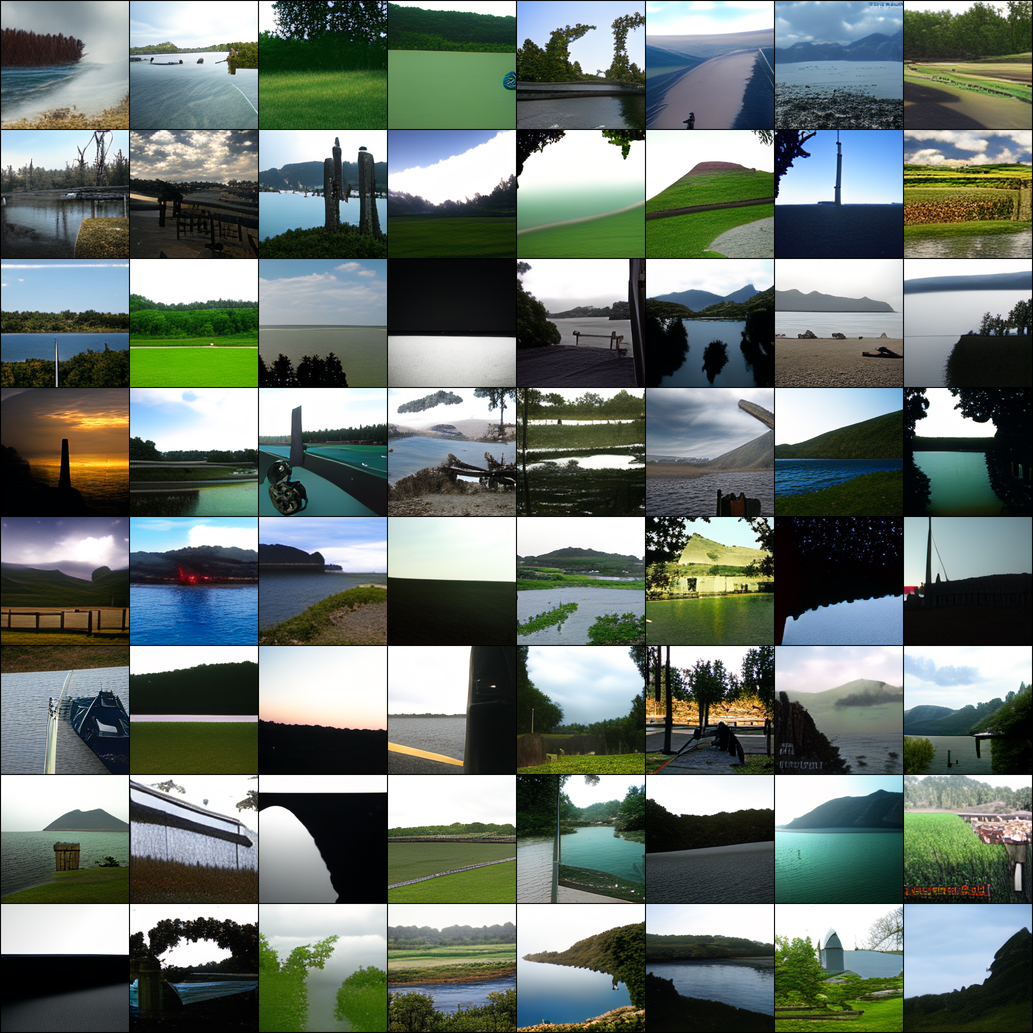
\includegraphics[width=1.0\textwidth]{figures/imagenet-lakeside-small.png}
        \caption{
            $256 \times 256$ successful samples from the class ``Lakeside''.
        }
    \end{subfigure}\\
    \vspace{0.5cm}
    \begin{subfigure}[b]{0.47\textwidth}
        \centering
        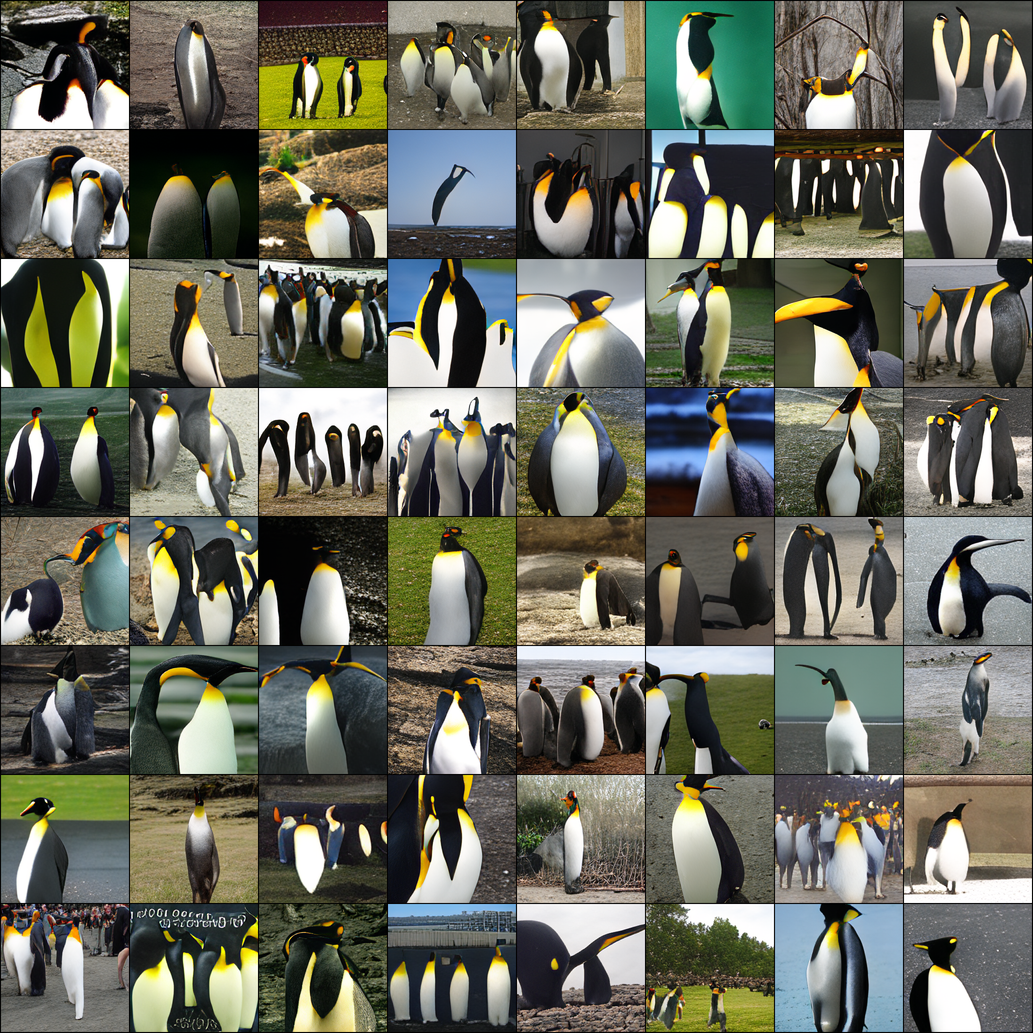
\includegraphics[width=1.0\textwidth]{figures/imagenet-penguin-small.png}
        \caption{
            $256 \times 256$ failed samples from the class ``King Penguin''.
        }
    \end{subfigure}
    \hfill
    \begin{subfigure}[b]{0.47\textwidth}
        \centering
        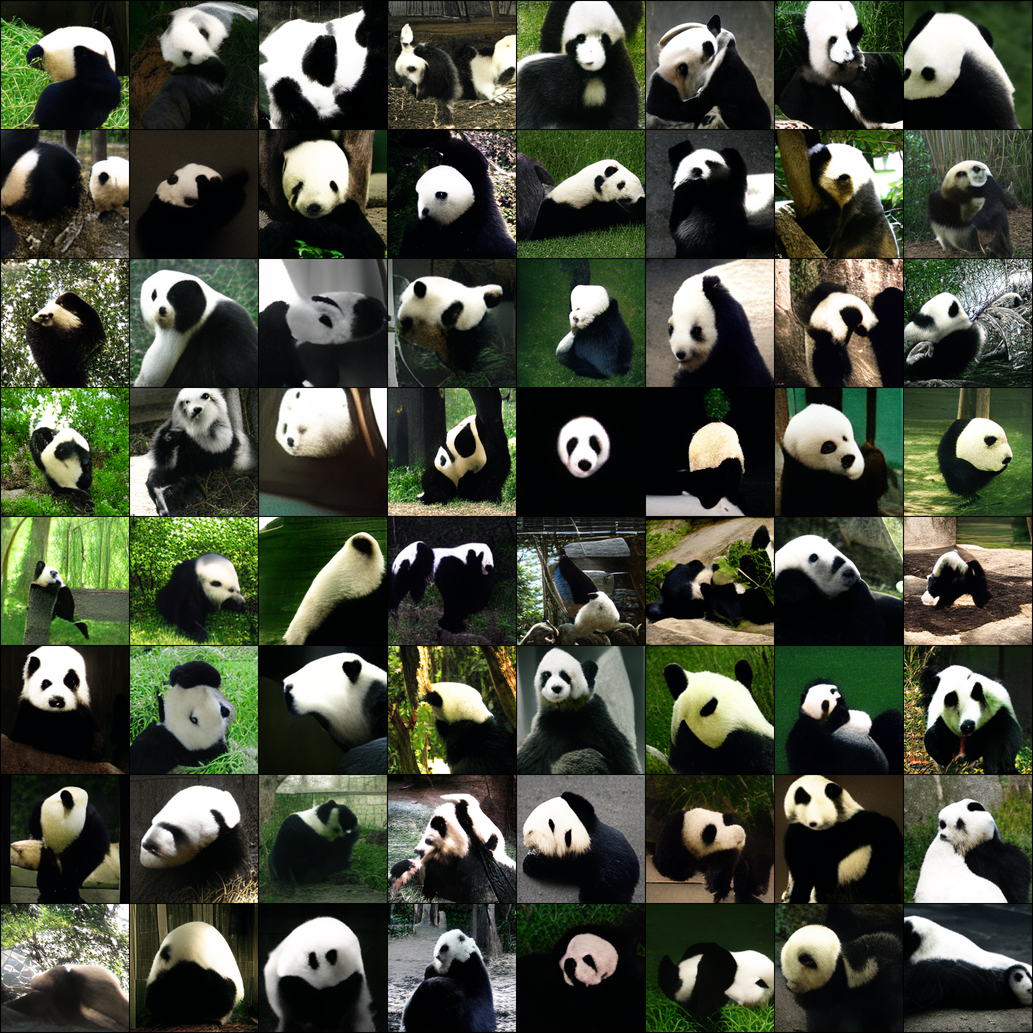
\includegraphics[width=1.0\textwidth]{figures/imagenet-panda-small.png}
        \caption{
            $256 \times 256$ failed samples from the class ``Giant Panda''.
        }
    \end{subfigure}
    \caption{Examples of class-conditioned generation on ImageNet using
        $\markovSteps = 50$ sampling steps. Top row contains examples of
    successful samples whereas bottom row showed failed samples. The contents of
    the failed samples nonetheless do resemble the target class.}
    \label{fig:imagenet}
\end{figure}

A relatively new method of providing a conditioning signal is to instead provide
natural language prompts, and learn the joint distribution of prompts and
images. At inference time, this allows for text-to-image generation which in
turn allows for zero-shot image generation given a sufficiently sized training
dataset. Most notably, DALL·E~\cite{ramesh2021dalle} and recently
DALL·E-2~\cite{ramesh2022dalle2}, with the former generating VQ-VAE discrete
latents and the latter generating continuous \textit{``CLIP Image embeddings''}.
DALL·E-2 was able to produce high fidelity samples at $1024 \times 1024$
resolution. Concurrently, Latent Diffusion
Models~\cite{rombach2021highresolution} used text embeddings to condition
sampling, again allowing for zero-shot generation. Our model is also capable of
using such methods, turning our model from an unconditional or class-conditioned
generative model to a text-to-image generative model. However, due to
time-constraints we did not experiment with this approach, leaving this for
future work.

\subsection{Arbitrary Image Inpainting}

As outlined earlier, \acrlong{nar} generative models have a number of advantages
on inpainting tasks, including supporting arbitrary masks and being able to use
the full context available to them. We provide a number of examples of
inpainting on FFHQ1024 and ImageNet, showcasing different patterns and different
results given the same starting image. As our method utilises a vector quantized
image model, it is incapable of doing fine-grained inpainting at a pixel level.
Nonetheless, the results show consistently good inpainting results when
operating at a \gls{vq} latent level.

\begin{figure}[ht]
    \centering
    \begin{subfigure}[b]{\textwidth}
        \centering
        \label{fig:inpaintExample}
        \includegraphics[width=1.0\linewidth]{figures/inpaint.png}
        \caption{A large example of inpainting on a $1024 \times 1024$ image using our
        model.}
    \end{subfigure}
    \\
    \begin{subfigure}[b]{0.47\textwidth}
        \centering
        \includegraphics[width=1.0\textwidth]{figures/inpaint-block/inpaint-variation-small.png}
        \caption{
            Multiple outputs of inpainting using the same block mask.
        }
    \end{subfigure}
    \hfill
    \begin{subfigure}[b]{0.47\textwidth}
        \centering
        \includegraphics[width=1.0\textwidth]{figures/inpaint-rand/inpaint-variation-small.png}
        \caption{
            Multiple outputs of inpainting on the same random mask. 
        }
    \end{subfigure}
    \caption{
        Inpainting results on FFHQ-1024. We compute multiple outputs per
        input image and mask to demonstrate diversity of outputs. Inpainting
        using a \gls{vq} image model cannot be applied perfectly at a
        pixel-level. Nevertheless, the model still produces many convincing
        outputs at very high resolutions.
    }
\end{figure}

